\documentclass[10pt]{beamer}

%STANDARD PREAMBLE
%https://tex.stackexchange.com/questions/68821/is-it-possible-to-create-a-latex-preamble-header
\usepackage{/Users/miw267/Repos/latex_preamble/beamer_preamble}
%\usepackage{/Users/miw267/Repos/csci246_spring2025/slides/preambles/beamer_preamble_for_CSCI246}


%%%
% SPECIFIC TO THIS DOCUMENT 
%%%
\usepackage{animate}


\newcommand{\kernel}{K}

%%%%
% DOCUMENT 
%%%
\title{04/16/2026: Coding Workshop: Attention}
\author{Reference: \textit{Dive Into Deep Learning}, Chapter 10.}
\date{CSCI 546: Diffusion Models}

\begin{document}
\maketitle

%\begin{frame}{Table of contents}
%  \setbeamertemplate{section in toc}[sections numbered]
%  \tableofcontents[hideallsubsections]
%\end{frame}

\begin{frame}{Table of contents}
  \setbeamertemplate{section in toc}[sections numbered]
  \setbeamertemplate{subsection in toc}[subsections numbered]
  \tableofcontents
\end{frame}





\section{Course Logistics}




\begin{frame}{Feedback on Reading Survey \#8}

The original question was:
\alert{What is attention, and how does it work?}

\vfill 

In general, people provided great answers to the first question, but many people struggled (or didn't answer) the second question.
\pause 
\vfill 
The easiest way to answer the second question is to reference the notion of keys, queries, and values.
\pause 
\vfill 
\colorbox{yellow!30}{\textbf{Poll.}} Would anybody like to give a verbal answer to the second question?

\end{frame}






\section{Coding Workshop}



\section{Mini-Lecture}


\begin{frame}[standout]
\alert{Attention as Nadaraya-Watson Kernel Regression}
\end{frame}



\begin{frame}{Nonparametric Regression}

Suppose we are given $n$ pairs of observations $(x_1,y_1),\hdots, (x_n,y_n)$.  \pause 

In \alert{non-parametric regression}, we want to model the \textbf{response variable} $Y$ as a function of \textbf{covariates} $X$ making a few assumptions as possible (e.g. without assuming linearity). \pause 

This allows us to perform regressions for datasets such as the Cosmic Microwave Background (CMB) radiation: 
\begin{figure} 
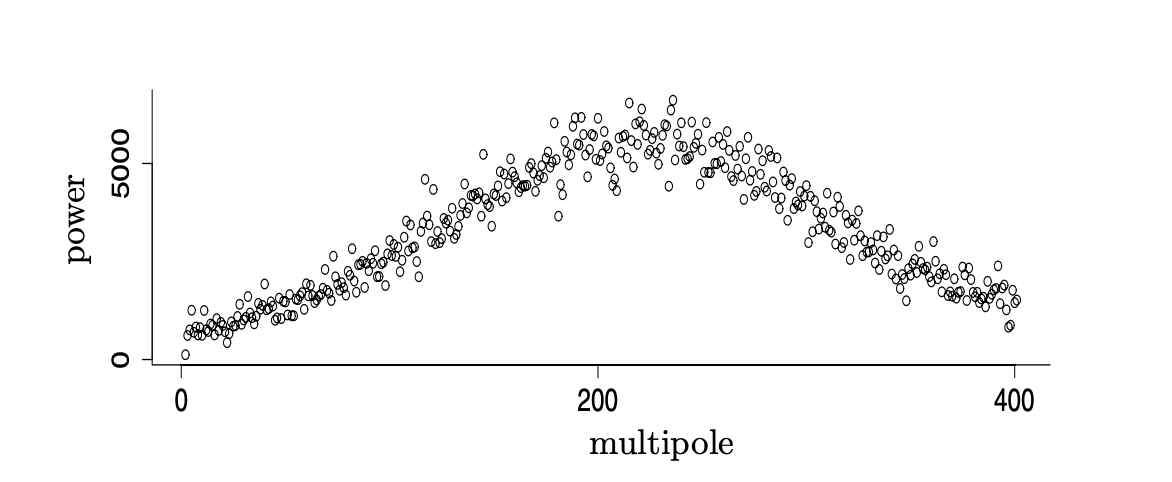
\includegraphics[width=.8\textwidth]{images/CMB} 
\end{figure}

\bottomtext{\hfill Reference: Wasserman, Larry. \textit{All of nonparametric statistics.}}
\end{frame}

\begin{frame}{Nonparametric Regression}

We assume the \textbf{response variable} $Y$ is related to known \textbf{covariates} $X=x$ by the equation
\[Y_i = r(x_i) + \epsilon_i, \qquad  \E[\epsilon_i]=0, \quad i=1,\hdots,n.\]
\pause
\vfill  
We may interpret the \qq{trend} $r(x)$ as the mean of $Y$ conditional on $X=x$, that is
\[ r(x) = \E[Y \mid X=x].\]
	
\end{frame}

\begin{frame}{Smoothing Kernel}

\only<1-2>{Smoothing kernels are for taking local averages.} \pause \only<2>{Examples:}

%\begin{figure} 
%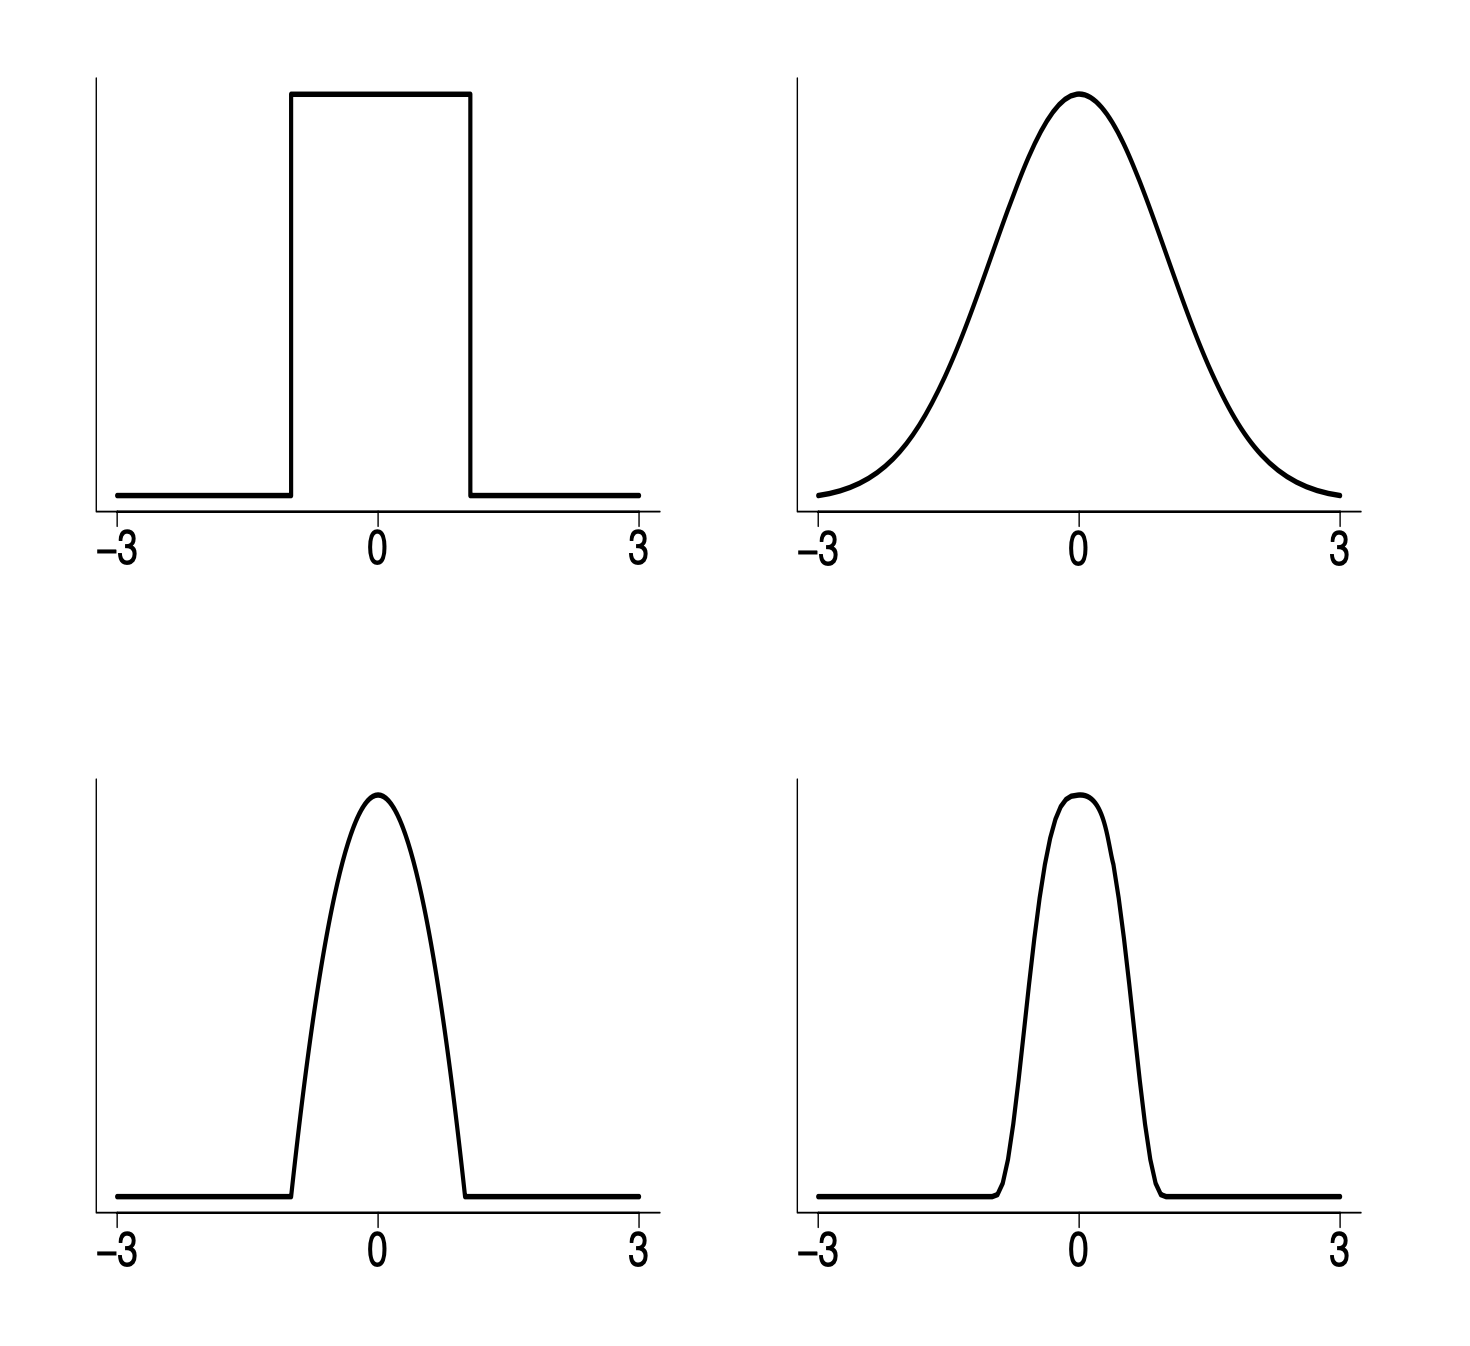
\includegraphics[width=.7\textwidth]{images/smoothing_kernel} 
%\end{figure}

\centering
\small 
\begin{tabular}{cc}

\begin{tabular}{c}
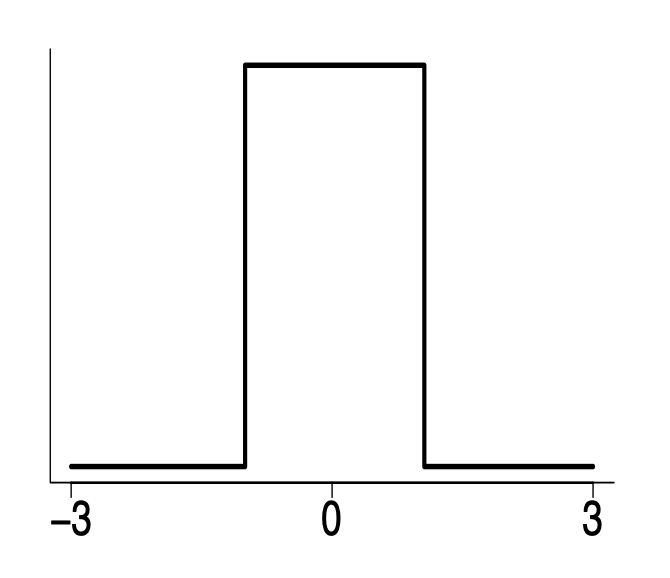
\includegraphics[width=0.25\textwidth]{images/boxcar}
\\
\textbf{Boxcar} \\
\only<3>{$\kernel(x)=\half \, I(x)$}
\end{tabular}
&
\begin{tabular}{c}

\includegraphics[width=0.25\textwidth]{images/gaussian}
\\
\textbf{Gaussian} \\
\only<3>{$\kernel(x)=\frac{1}{\sqrt{2\pi}} e^{-x^2/2}$}
\end{tabular}

\\[1.5em]

\begin{tabular}{c}
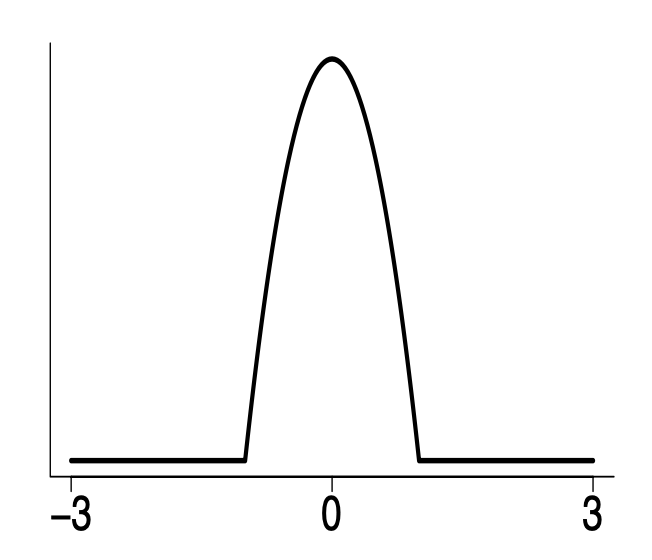
\includegraphics[width=0.25\textwidth]{images/epanechnikov}
\\
\textbf{Epanechnikov} \\
\only<3>{$\kernel(x)=\frac{3}{4} (1-x^2)\, I(x)$}
\end{tabular}
&
\begin{tabular}{c}
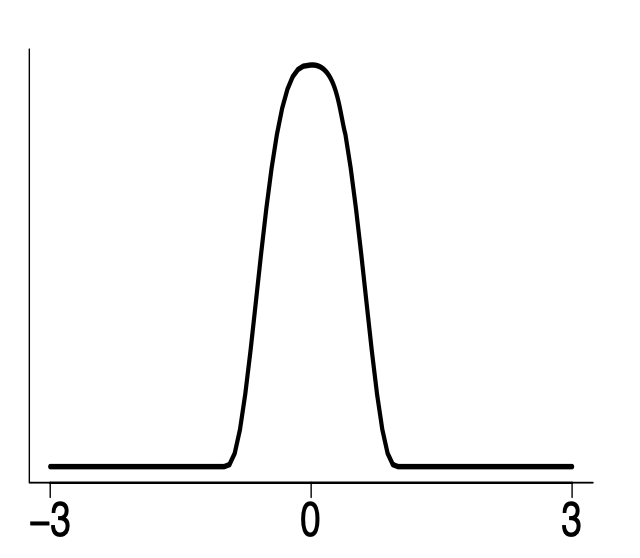
\includegraphics[width=0.25\textwidth]{images/tricube}
\\
\textbf{Tricube} \\
\only<3>{$\kernel(x)=\frac{70}{81} (1-|x|^3)^3 \, I(x)$} 
\end{tabular}
\end{tabular}

\only<3>{
\begin{align*}
I(x) =
 \begin{cases}
1, & \text{if} \; |x| \leq 1 \\
0, & \text{if} \; |x| > 1 	
\end{cases}
\end{align*}
}

\only<1-2>{\bottomtext{\hfill Reference: Wasserman, Larry. \textit{All of nonparametric statistics.}}}
\end{frame}

\begin{frame}{Smoothing Kernel}

\begin{mybluebox}[title=Definition]
A \textbf{smoothing kernel} is any smooth function $\kernel$ such that $\kernel(x)>0$ and
%
\begin{align*}
\int \kernel(x) \text{d}x=1, \qquad 	\int x \, \kernel(x) \text{d}x=0, \quad \text{and} \quad \sigma^2_\kernel \defeq \int x^2 \kernel(x) \text{d}x >0 
\end{align*}
\end{mybluebox}

\pause 
\colorbox{yellow!30}{\textbf{Poll.}} What's an easy way to construct a smoothing kernel?

\pause 
\vfill 
\colorbox{green!30}{\textbf{Solution.}} Just take the p.d.f. of a (non-degenerate) random variable with mean 0.



\bottomtext{Reference: Wasserman, Larry. \textit{All of nonparametric statistics.}}
\end{frame}




%\begin{frame}{Estimating the trend}
%	
%\begin{mybluebox}[title=Definition]
%
%\only<1->{An estimator $\widehat{r}$ of the trend $r$ is a \textbf{linear smoother} if it can be written as}
%%
%\only<1>{
%\begin{align*}
%\widehat{r}(x) = \sum_{i=1}^n \ell_i(x) y_i
%\end{align*}
%}
%
%\only<2->{
%\begin{align*}
%\widehat{r}(x) = \sum_{i=1}^n \; \explaintermbrace{weight}{\ell_i(x)} \explaintermbrace{observation}{y_i}
%\end{align*}
%}
%
%\end{mybluebox}
%
%\only<3>{
%\vfill
%Basically, we estimate the trend $r(x)$ by taking a weighted average of the $y_i$'s, giving higher weight to those points that are \qq{close} to $x$. 
%}
%
%
%\end{frame}


\begin{frame}{Estimating the trend}
	
\begin{mybluebox}[title=Definition]

\only<1->{The \textbf{Nadaraya-Watson kernel estimator} is defined by}
%
\only<1>{
\begin{align*}
\widehat{r}(x) = \sum_{i=1}^n w_i(x) y_i
\end{align*}
}

\only<2->{
\begin{align*}
\widehat{r}(x) = \sum_{i=1}^n \; \explaintermbrace{weight}{w_i(x)} \explaintermbrace{observation}{y_i}
\end{align*}
}

\only<3->{
where the weights $w_i(x)$ are given by
%
\begin{align}
w_i(x) = \frac{\kernel(\frac{x-x_i}{h})}{\sum_{j=1}^n \kernel(\frac{x-x_j}{h})}	
\end{align}
for a smoothing kernel $\kernel$ with  \textbf{bandwidth} $h>0$.
}
\end{mybluebox}

\only<4>{
\colorbox{yellow!30}{\textbf{Poll.}} Who can explain what's going on here?
}

\only<5->{
\vfill
\colorbox{blue!30}{\textbf{Remark.}} Basically, we estimate the trend $r(x)$ by taking a weighted average of the observations ($y_i$)'s, giving higher weight to the observations that are \qq{close} to $x$. 
} \only<6->{The larger the bandwidth $h$, the more observations that are considered   \qq{close}.
}

\end{frame}

\begin{frame}{Example: CMB Data}
Let's use Nadayara-Watson kernel regression to estimate the trend for CMB data.

\begin{figure} 
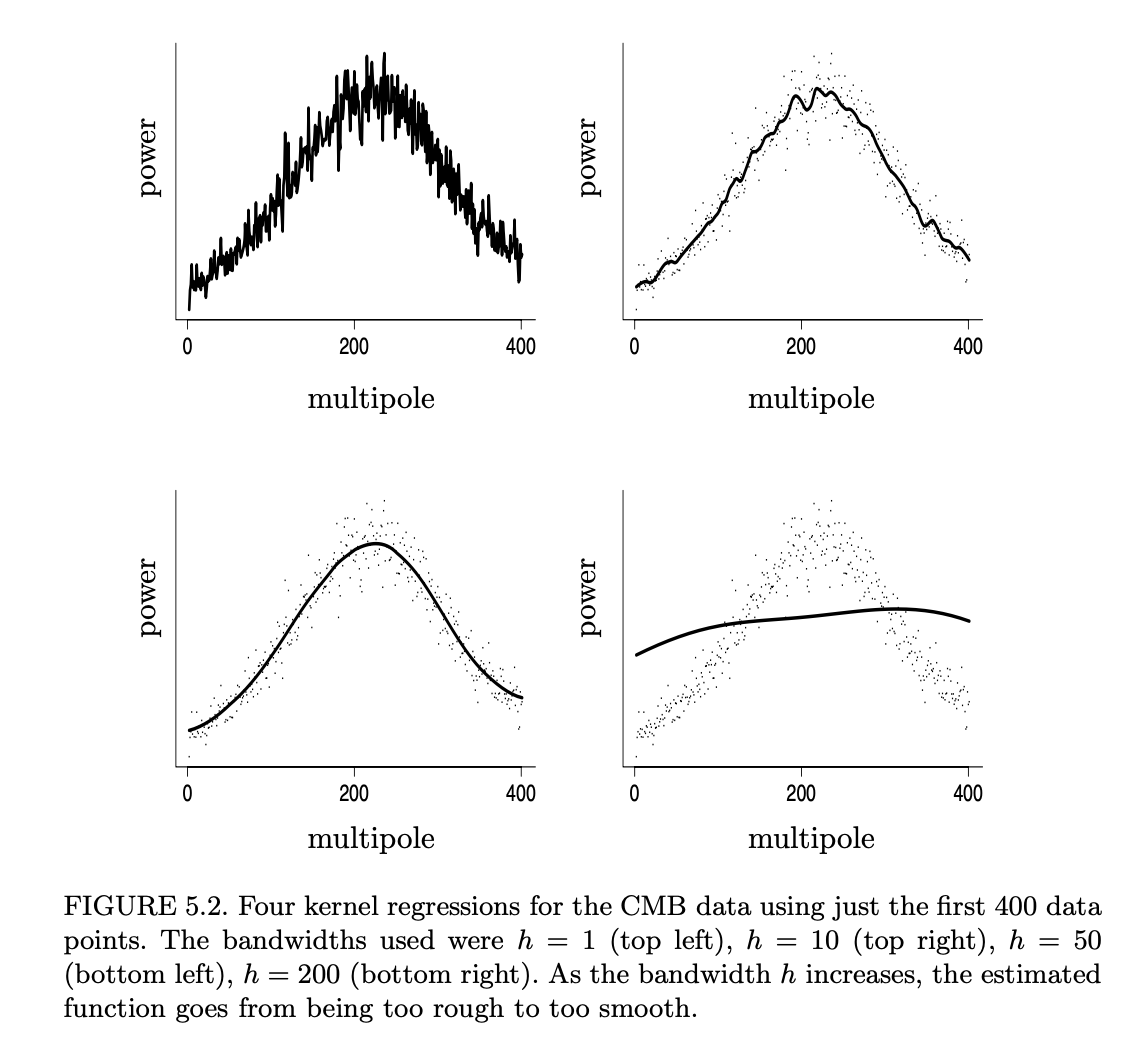
\includegraphics[width=.6\textwidth]{images/CMB_kernel_regression} 
\end{figure}	
\pause 
\colorbox{blue!30}{\textbf{Remark.}} The optimal bandwidth can be chosen via cross-validation.
\end{frame}



\begin{frame}[standout]

\alert{Discussion:} How is attention pooling related to Nadayara-Watson kernel regression?
\end{frame}
t
%
%\begin{frame}{Summary}
%
%Attention is Nadaraya–Watson with kernel
%
%\[ \kernel(k; q_j)=\exp(k \cdot q_j).\]
%
%\pause 
%\vfill 
%
%This kernel is \alert{learned} rather than fixed in advance.
%
%	
%\end{frame}


\begin{frame}{Attention as Nadaraya-Watson}
	
\begin{mybluebox}[title=Observation]

\only<1->{Attention can be expressed as}
%%
%\only<1>{
%\begin{align*}
%\Delta y_j = \sum_{i=1}^n w(k_i) y_i
%\end{align*}
%}
\only<1->{
\begin{align*}
\explaintermbrace{change in embedding}{\Delta y_j} = \sum_{i=1}^n \; \explaintermbrace{weight}{w_j(k_i)} \explaintermbrace{value (for $y_i$)}{v_i}
\end{align*}
}

\only<2->{
where the weights $w_j$ are given by
%
\begin{align}
w_j(k_i) = \frac{\exp ( q_j \cdot k_i / \sqrt{d} )}{\sum_{i'=1}^n \exp ( q_j \cdot k_{i'} / \sqrt{d} ) }	
\end{align}
}
\end{mybluebox}

\only<3->{
\colorbox{yellow!30}{\textbf{Poll.}} How is attention pooling related to Nadayara-Watson kernel regression?
}

\only<4->{
\vfill
\begin{itemize}
\item This kernel is \alert{learned} rather than fixed in advance. \pause
\item Each unit $j$ gets its \alert{own} kernel.
\item [...] 	
\end{itemize}

} 

\end{frame}

\end{document}

